%%%%%%%% ICML 2023 EXAMPLE LATEX SUBMISSION FILE %%%%%%%%%%%%%%%%%

\documentclass[nohyperref]{article}

% Recommended, but optional, packages for figures and better typesetting:
\usepackage{microtype}
\usepackage{graphicx}
\usepackage{subfigure}
\usepackage{booktabs} % for professional tables

% hyperref makes hyperlinks in the resulting PDF.
% If your build breaks (sometimes temporarily if a hyperlink spans a page)
% please comment out the following usepackage line and replace
% \usepackage{icml2023} with \usepackage[nohyperref]{icml2023} above.
\usepackage{hyperref}


% Attempt to make hyperref and algorithmic work together better:
\newcommand{\theHalgorithm}{\arabic{algorithm}}

% Use the following line for the initial blind version submitted for review:
\usepackage[accepted]{icml2023}

% If accepted, instead use the following line for the camera-ready submission:
% \usepackage[accepted]{icml2022}

% For theorems and such
\usepackage{amsmath}
\usepackage{amssymb}
\usepackage{mathtools}
\usepackage{amsthm}

% if you use cleveref..
\usepackage[capitalize,noabbrev]{cleveref}

%%%%%%%%%%%%%%%%%%%%%%%%%%%%%%%%
% THEOREMS
%%%%%%%%%%%%%%%%%%%%%%%%%%%%%%%%
\theoremstyle{plain}
\newtheorem{theorem}{Theorem}[section]
\newtheorem{proposition}[theorem]{Proposition}
\newtheorem{lemma}[theorem]{Lemma}
\newtheorem{corollary}[theorem]{Corollary}
\theoremstyle{definition}
\newtheorem{definition}[theorem]{Definition}
\newtheorem{assumption}[theorem]{Assumption}
\theoremstyle{remark}
\newtheorem{remark}[theorem]{Remark}

% Todonotes is useful during development; simply uncomment the next line
%    and comment out the line below the next line to turn off comments
%\usepackage[disable,textsize=tiny]{todonotes}
\usepackage[textsize=tiny]{todonotes}


% The \icmltitle you define below is probably too long as a header.
% Therefore, a short form for the running title is supplied here:
\icmltitlerunning{SL Project Checkpoint}

\newcommand{\dnl}{\mbox{}\par}
\newcommand{\mycomment}[1]{\textbf{Note:} \textit{#1}}
\newcommand{\cnote}[1]{\textsf{\color{blue} [#1]}}
%\newcommand{\cnote}[1]{}


\begin{document}

\twocolumn[
\icmltitle{CS5033 - SL Project Checkpoint}

% It is OKAY to include author information, even for blind
% submissions: the style file will automatically remove it for you
% unless you've provided the [accepted] option to the icml2022
% package.

% List of affiliations: The first argument should be a (short)
% identifier you will use later to specify author affiliations
% Academic affiliations should list Department, University, City, Region, Country
% Industry affiliations should list Company, City, Region, Country

% You can specify symbols, otherwise they are numbered in order.
% Ideally, you should not use this facility. Affiliations will be numbered
% in order of appearance and this is the preferred way.
\icmlsetsymbol{equal}{*}

\begin{icmlauthorlist}
\icmlauthor{Airi Shimamura}{} %{equal,yyy}
\icmlauthor{Khoi Trinh}{} %{equal,yyy,comp}
%\icmlauthor{Firstname3 Lastname3}{comp}
%\icmlauthor{Firstname4 Lastname4}{sch}
%\icmlauthor{Firstname5 Lastname5}{yyy}
%\icmlauthor{Firstname6 Lastname6}{sch,yyy,comp}
%\icmlauthor{Firstname7 Lastname7}{comp}
%\icmlauthor{}{sch}
%\icmlauthor{Firstname8 Lastname8}{sch}
%\icmlauthor{Firstname8 Lastname8}{yyy,comp}
%\icmlauthor{}{sch}
%\icmlauthor{}{sch}
\end{icmlauthorlist}

%\icmlaffiliation{yyy}{Department of XXX, University of YYY, Location, Country}
%\icmlaffiliation{comp}{Company Name, Location, Country}
%\icmlaffiliation{sch}{School of ZZZ, Institute of WWW, Location, Country}

%\icmlcorrespondingauthor{Amy McGovern}{first1.last1@xxx.edu}
%\icmlcorrespondingauthor{Anna Partner}{first2.last2@www.uk}

% You may provide any keywords that you
% find helpful for describing your paper; these are used to populate
% the "keywords" metadata in the PDF but will not be shown in the document
%\icmlkeywords{Machine Learning, ICML}

\vskip 0.3in
]

% this must go after the closing bracket ] following \twocolumn[ ...

% This command actually creates the footnote in the first column
% listing the affiliations and the copyright notice.
% The command takes one argument, which is text to display at the start of the footnote.
% The \icmlEqualContribution command is standard text for equal contribution.
% Remove it (just {}) if you do not need this facility.

%\printAffiliationsAndNotice{}  % leave blank if no need to mention equal contribution
%\printAffiliationsAndNotice{\icmlEqualContribution} % otherwise use the standard text.

\section*{Introduction}

For our Supervised Learning project this semester, we want to create a few models to predict a user's preference for a song on the Spotify streaming platform.

Each song on Spotify have their own set of 11 features. These features are: danceability, energy, key, loudness, mode, speechiness, acousticness, instrumentalness, liveness, valence, and tempo.

A user can request their streaming history from Spotify via the P rivacy section of their account. For the purpose of this project, Khoi's one-year streaming history from February 2022 
to February 2023 will be used as the 1 class, for songs we like; and about 4200 random songs which Khoi has never heard will be used as the 0 class, for songs we do not like.

The dataset has 56,210 songs in class 1, and 4,170 songs in class 0. However, the songs in class 1 have duplicates, due to the nature of streaming a song multiple times.
We expect this number will be much lower once the duplicates are removed.

\section{Hypotheses}
Our first hypothesis is that our supervised learning models will be able to classified these songs as likes or dislikes with at least 90\% accuracy.

Our second hypothesis is that out of the four chosen algorithms; Random Forest will give us the best performance; followed by Decision Tree, then Logistic Regression, and finally Naive Bayes. We will evaluate each algorithm's performance by comparing the value of Precision, Recall, and produce ROC curves for each algorithm.

\section{Experimental Progress}

\subsection{Data Preprocessing}

For the preprocessing of the data, we removed duplicates, the preference column, as well as scaling and shuffling the data before passing into the model.

\subsection{Khoi's Progress}

For this project, Khoi is implementing two methods: logistic regression and decision trees.

Logistic Regression is a statistical machine learning algorithm predicting the probability of a target variable by fitting a logistic function to the input features. This optimizes the parameters of the logistic function by minimizing the cost function, which measures the difference between the predicted probabilities and the actual class labels.

Decision Tree is a machine learning algorithm to predict the class of an input based on its features. This algorithm partitions the input space into increasingly smaller regions based on the values of the input features by selecting the features and test conditions that best separate the training data into the different classes. This process is repeated recursively to create a tree-like structure until a final decisionis made.

Currently, he is working on the logistic regression model.

For the model, Khoi is consider the learning rate $\alpha = 0.01$ and the model will train for 1000 iterations. Moreover, he implemented the sigmoid, logistic loss, and gradient fucntion from scratch. After one run, here are his results:

Precision: 94.56\%

Recall: 49.18\%

Accuracy: 96.83\%

Along with this ROC curve

\begin{figure}[H] %h forces the figure to be inserted right here
    \centering
    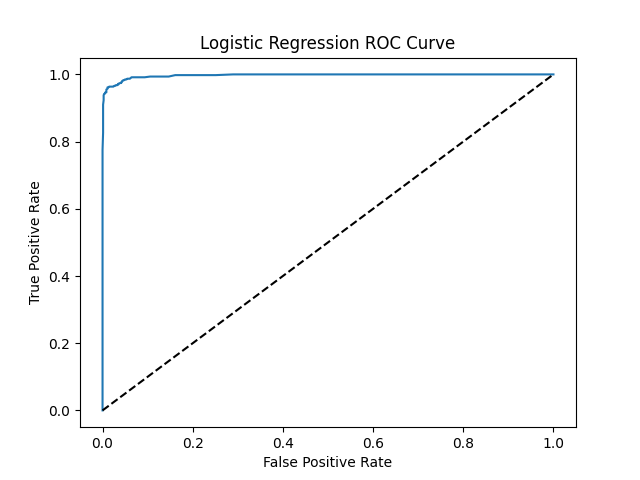
\includegraphics[width=0.75\linewidth]{LogisticROC.png}
    \caption{ROC Curve for Logistic Regression}
\end{figure}

\subsection{Airi's Progress}

For this project, Airi is implementing two methods: naive bayes and random forest.

Naive Bayes is a group of probabilistic machine learning algorithms based on applying Bayes' theorem with the assumption of independence between features. This assumes that the presence or absence of one feature does not affect the presence or absence of any other feature within a class, and calculates the probabilities of each class label given the values of the features from the input. The class with the highest probability is then selected as the predicted class label for the given input.

Random Forest is an ensemble learning method that combines multiple decision trees to improve the performance and reduce overfitting. Each decision tree is constructed by randomly selecting a set of features and samples from the training set. This randomization helps to make a model less sensitive to noise and outliers in the data, and outperforms other algorithms.

For the random forest model, Airi used the Gini index as the criterion for tree splitting with 20 decision trees, and the Naive Bayes model was implemented based on the Bayes' theorem. Also, to evaluate the performance of the models, precision, accuracy, and recall were calculated and both of the models achieved high scores as follows

— Random Forest:
Accuracy: 97.91\%
Precision: 97.41\% 
Recall: 49.29\%

— Naive Bayes: 
Accuracy:  97.68\%	
Precision: 97.78\% 
Recall: 49.04\% 


\section{Experimental Results and Analysis}

\subsection{Khoi's Results}

For this project, Khoi implemented logistic regression and decision tree.

\textbf{Logistic Regression} is a statistical machine learning algorithm predicting the probability of a target variable by fitting a logistic function to the input features. This optimizes the parameters of the logistic function by minimizing the cost function, which measures the difference between the predicted probabilities and the actual class labels.

For this model, Khoi implemented the following functions:

Sigmoid/Logistic function: $\sigma(z) = \frac{1}{1 + e^{-z}}$

% j = -1/m * (y.T.dot(np.log(h + eps)) + (1-y).T.dot(np.log(1-h + eps)))
Logistic loss function: $log loss = \Sigma_{x, y \in D} -ylog(y') - (1 - y)log(1 - y')$

Where:

$(x, y) \in D$ is the data set containing labeled instances.

$y$ is the label in a labeled example; in this case, it is either 0 or 1.

$y'$ is the predicted value, given the features in x.

Khoi also implemented the logistic regression function from scratch, and can be seen in the code provided.

Here are the results, with $\alpha = 0.5$ and 1000 iterations.

Accuracy: 97.6\%

Precision: 96.19\%

Recall: 97.22\%

\textbf{Decision Tree} is a machine learning algorithm to predict the class of an input based on its features. This algorithm partitions the input space into increasingly smaller regions based on the values of the input features by selecting the features and test conditions that best separate the training data into the different classes. This process is repeated recursively to create a tree-like structure until a final decision is made.

Similar to the previous model, Khoi implemented this from scratch, and can be seen in the provided code. The criteria Khoi is using to split the node is the Gini impurity. This is a measure of the impurity or randomness of a set of examples used in decision trees. It measures the probability that two randomly chosen examples from the set have different class labels. The aim is to find the split that results in the lowest Gini impurity of the resulting subsets.

Here are the results, with a tree depth of 5:

Accuracy: 98.07\%

Precision: 97.02\%

Recall: 97.64\%

\subsection{Airi's Results}

\subsection{Hypothesis 1}

\subsection{Hypothesis 2}


\section{Difficulties Encountered}

The ROC curves for the Naive Bayes, Decision Trees, and Random Forest are all straight lines, which indicates the models cannot identify any relevant patterns or features, so either the data processing or the models need to be re-evaluated.

Moreover, Naive Bayes performance is much better than Logistic Regression and Random Forest; so all of these models will need to be re-evaluated.

\section{Future Work}

Khoi will continue refinding his logistric regression model, as well as work on the decision tree model. The decision tree model will be useful for random forest, as well.

%\cnote{All written proposals must be no longer than one page per number of people in the group.}

\bibliographystyle{mslapa}
\bibliography{my,book}

\end{document}


% This document was modified from the file originally made available by
% Pat Langley and Andrea Danyluk for ICML-2K. This version was created
% by Iain Murray in 2018, and modified by Alexandre Bouchard in
% 2019 and 2021 and by Csaba Szepesvari, Gang Niu and Sivan Sabato in 2022. 
% Previous contributors include Dan Roy, Lise Getoor and Tobias
% Scheffer, which was slightly modified from the 2010 version by
% Thorsten Joachims & Johannes Fuernkranz, slightly modified from the
% 2009 version by Kiri Wagstaff and Sam Roweis's 2008 version, which is
% slightly modified from Prasad Tadepalli's 2007 version which is a
% lightly changed version of the previous year's version by Andrew
% Moore, which was in turn edited from those of Kristian Kersting and
% Codrina Lauth. Alex Smola contributed to the algorithmic style files.
